\documentclass[acmsmall,nonacm]{acmart}
\setcopyright{none}
\settopmatter{printacmref=false,printfolios=true}
\acmDOI{}
\acmYear{2026}
\copyrightyear{2026}
\acmConference[]{}{}{}
\acmBooktitle{}
\acmISBN{}
\usepackage{booktabs}
\usepackage{tabularx}
\usepackage{array}
\usepackage{graphicx}
\usepackage{enumitem}
\usepackage{microtype}
\setlength{\headheight}{18.5pt}
\usepackage{url}
\newcolumntype{Y}{>{\raggedright\arraybackslash}X}
\newcommand{\etal}{\textit{et al.}}
\begin{document}

\title{Evaluating Multilingual Reliability of Large Language Models in Scientific Literature Analysis: A Review of Methods, Evidence, and Open Problems}

\author{Sanjit Nayyar}
\authorsaddresses{}

\begin{abstract}
Large language models (LLMs) are increasingly embedded in the scientific workflow, assisting with literature screening, summarization, question answering, and cross-lingual translation of research articles \cite{Scherbakov2025,Kleidermacher2025}. Because the vast majority of indexed scientific output is published in English while many researchers are not native English speakers \cite{Kleidermacher2025,Amano2023}, multilingual LLMs are frequently proposed as a route toward broader access to scientific knowledge. Yet reliability is not uniform across languages: multilingual benchmarks report differences in accuracy, factuality, and confidence estimation between English and lower-resource or typologically different languages \cite{Xuan2025,Xue2024,GarcíaFerrero2024}. This review synthesizes recent empirical and methodological literature on multilingual reliability in scientific-literature-facing LLM applications. It examines mechanisms associated with cross-lingual unreliability, including uneven pretraining resources, translation-mediated information loss, terminology mismatch, and language-specific hallucination; compares mitigation strategies such as retrieval-augmented generation, multilingual factuality evaluation, cross-lingual reasoning, and domain adaptation; and identifies limitations in current evaluation and deployment practice. The review argues that reliability should be treated as an end-to-end property of multilingual literature-analysis workflows rather than as a single model score. Major unresolved issues include standardized task-realistic evaluation, genuinely low-resource language coverage, multilingual-native retrieval, calibration and uncertainty communication, structural bias, and human-in-the-loop verification.
\end{abstract}

\ccsdesc[500]{Computing methodologies~Natural language processing}
\ccsdesc[300]{Information systems~Information retrieval}
\ccsdesc[200]{Information systems~Digital libraries and archives}
\keywords{large language models, multilingual natural language processing, scientific literature analysis, hallucination, factuality, cross-lingual evaluation, retrieval-augmented generation, low-resource languages}
\maketitle

\section{Introduction}\label{sec:introduction}
Large language models (LLMs) such as GPT-4, LLaMA, and BLOOM have moved from general-purpose assistants into specialized roles within the scientific research pipeline \cite{OpenAI2023,Touvron2023,BigScience2022}. These roles include screening titles and abstracts for systematic reviews, extracting structured data from full-text articles, summarizing findings across large corpora, answering domain-specific questions, and translating research output for readers who do not work primarily in English \cite{Scherbakov2025,Kleidermacher2025}. Reviews of review-automation literature show that LLMs are already being evaluated across several stages of evidence synthesis, although the evidence base remains dominated by English-language workflows \cite{Scherbakov2025}.

The appeal of multilingual systems is closely connected to the language structure of scientific communication. English dominates indexed scientific publishing, while non-native English speakers report additional time and participation costs across reading, writing, and dissemination activities \cite{Amano2023}. LLM-based translation and summarization therefore have potential to reduce language barriers; recent work has demonstrated large-scale translation of scientific articles into multiple languages while preserving structured markup, while multilingual medical question-answering and reasoning benchmarks have expanded the empirical evidence base \cite{Kleidermacher2025,GarcíaFerrero2024,Xuan2025}. However, accessibility alone does not establish reliability.

In this review, \emph{multilingual reliability} refers to the extent to which an LLM produces accurate, factually grounded, appropriately calibrated, complete, and traceable outputs across languages when performing scientific-literature-analysis tasks. The definition is deliberately broader than task accuracy: a system can answer correctly on average while still being overconfident, omit important evidence, mistranslate technical terminology, or produce unsupported claims. This distinction matters in scientific literature analysis because errors can propagate across retrieval, screening, extraction, synthesis, and reporting stages.

Multiple independent benchmarks converge on a language-dependent performance pattern. Accuracy can decline as evaluation moves away from English toward lower-resource or typologically different languages, while hallucination and confidence estimation can also vary by language \cite{Xuan2025,Xue2024,GarcíaFerrero2024,Huang2025}. At the same time, the literature is heterogeneous: some interventions improve specific tasks, and language-context matching can improve calibration for culturally or geographically specific questions \cite{Xue2024}. The central problem is therefore not whether multilingual LLMs are useful, but under what conditions their outputs can be considered reliable enough for scientific evidence workflows.

This review focuses on multilingual reliability specifically in scientific and biomedical literature-facing applications, while drawing on general multilingual benchmarks and hallucination research where these provide mechanisms or evaluation evidence relevant to scientific use. It does not attempt to rank individual commercial models or provide a systematic meta-analysis of effect sizes. Instead, it synthesizes the evidence thematically around performance disparities, sources of cross-lingual unreliability, hallucination and factuality, calibration, translation and terminology, and scientific literature-analysis applications.

This review makes four contributions: (1) it synthesizes evidence on multilingual reliability across scientific and biomedical literature-analysis tasks; (2) it organizes the major mechanisms associated with cross-lingual degradation; (3) it compares current mitigation strategies and their limitations; and (4) it identifies research gaps and directions for developing more reliable multilingual scientific-literature workflows. The remainder of the paper preserves the seven-section structure of the cleaned manuscript: Section~\ref{sec:background} establishes background and related work; Section~\ref{sec:mechanisms} develops the main thematic discussion; Section~\ref{sec:approaches} surveys mitigation approaches; Section~\ref{sec:challenges} discusses limitations; Section~\ref{sec:gaps} identifies research gaps; and Section~\ref{sec:conclusion} concludes.

\begin{figure*}[t]
\centering
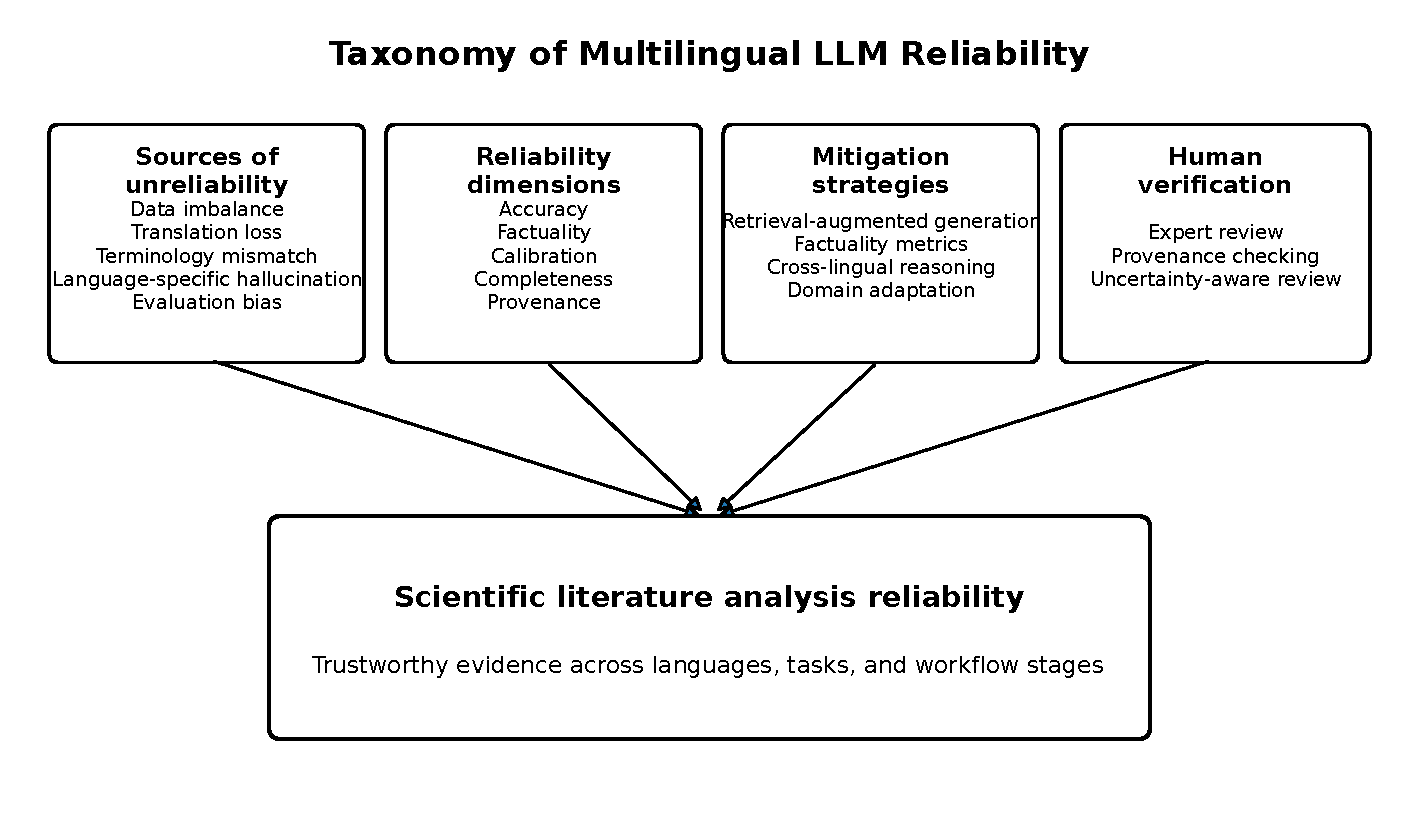
\includegraphics[width=0.96\textwidth]{figures/fig1_taxonomy.pdf}
\Description{A four-part taxonomy showing sources of unreliability, reliability dimensions, mitigation strategies, and human verification surrounding scientific literature analysis reliability.}
\caption{Taxonomy of multilingual LLM reliability. Reliability is treated as the interaction of sources of unreliability, observable reliability dimensions, mitigation strategies, and human verification.}
\label{fig:taxonomy}
\end{figure*}

\section{Background and Related Work}\label{sec:background}
\subsection{Multilingual Models and Evaluation Benchmarks}
Multilingual capability in LLMs has developed through several architectural generations. Early multilingual pretrained transformers such as mT5 extended the text-to-text framework across 101 languages using a Common Crawl-derived corpus and demonstrated competitive performance on multilingual benchmark suites \cite{Xue2021,Hu2020}. BLOOM subsequently scaled this approach to 176 billion parameters and was trained on the ROOTS corpus covering many natural and programming languages through a large international collaboration \cite{BigScience2022}. More recent general-purpose systems, including LLaMA and GPT-4, were not designed exclusively as multilingual scientific models but exhibit multilingual competence as a consequence of large-scale pretraining \cite{Touvron2023,OpenAI2023}.

A comprehensive survey of multilingual LLMs organizes the field around alignment strategies intended to transfer capability across languages and identifies persistent asymmetries associated with available training resources \cite{Qin2025}. The relevant implication for scientific literature analysis is that multilingual capability should not be interpreted as uniform capability: the existence of a multilingual model does not guarantee equal performance across languages, domains, or tasks.

The evaluation of multilingual LLMs has matured alongside the models themselves. XTREME established an early cross-lingual benchmark spanning 40 languages and 9 tasks, showing both strong English performance and substantial variation across languages \cite{Hu2020}. More recent benchmarks have targeted reasoning and knowledge capabilities of contemporary LLMs. MMLU-ProX extends MMLU-Pro to 29 languages using translated questions with expert review and reports substantial cross-language differences in accuracy \cite{Xuan2025}. Domain-specific benchmarks reveal comparable patterns: MedExpQA reports lower performance for French, Italian, and Spanish than for English across the evaluated LLM settings \cite{GarcíaFerrero2024}.

Confidence estimation provides a complementary dimension. MlingConf evaluates multilingual confidence estimation and reports a language-dominance effect for language-agnostic tasks, while language-specific prompting can improve reliability on culturally or geographically specific tasks \cite{Xue2024}. These benchmarks are not themselves scientific-literature workflows, but they provide evidence about mechanisms that can affect downstream scientific use.

\subsection{Hallucination and Literature-Review Applications}
Underlying much of the multilingual reliability literature is hallucination: the production of fluent content that is factually incorrect or unsupported by a source \cite{Ji2023,Huang2025}. The literature distinguishes factuality-oriented errors from faithfulness errors relative to a provided source and surveys mitigation approaches spanning training, retrieval, and post-hoc correction \cite{Huang2025}. Multilingual evidence indicates that hallucination behavior can differ across languages, making language a relevant reliability variable rather than merely a presentation choice \cite{Huang2025}.

A parallel line of research has evaluated LLMs directly within systematic-review and evidence-synthesis pipelines. Scherbakov \etal.\ reviewed the emerging literature and identified title/abstract screening as a frequent automation target, while Delgado-Chaves \etal.\ found that LLMs can reduce screening workload but that performance depends on how inclusion and exclusion criteria are specified \cite{Scherbakov2025,DelgadoChaves2025}. Much of this evidence concerns English-language corpora and prompting, leaving a central question: how do these workflows behave when source retrieval, screening, extraction, reasoning, or output occurs across multiple languages? This review connects the multilingual benchmark evidence to that workflow-level question.

\section{Main Thematic and Technical Discussion: Mechanisms of Multilingual Unreliability}\label{sec:mechanisms}
Figure~\ref{fig:taxonomy} summarizes the conceptual organization used in this section. Rather than treating each study independently, the evidence is grouped by the mechanisms through which multilingual reliability can degrade.

\subsection{Cross-Lingual Performance and Hallucination}
The most consistent finding across multilingual benchmarks is that performance varies substantially by evaluation language. MMLU-ProX reports large within-model differences across its 29 languages, while MedExpQA similarly reports lower performance in several non-English settings \cite{Xuan2025,GarcíaFerrero2024}. XTREME likewise demonstrated wide variation across languages even when evaluating a common multilingual architecture \cite{Hu2020}. These results suggest that multilingual capability is better represented as a distribution over languages than as a single model-level property.

The evidence also indicates that the gap is not reducible to knowledge access alone. Table~\ref{tab:literature-comparison} summarizes the principal multilingual reliability studies retained in this review. In MedExpQA, performance differences persist in settings involving retrieved medical knowledge, pointing to a role for language-specific comprehension and reasoning as well as retrieval \cite{GarcíaFerrero2024}. For scientific literature analysis, this distinction is important because adding more documents does not automatically solve errors introduced during language processing or reasoning.

Beyond raw accuracy, the character and rate of model errors can differ across languages. Multilingual hallucination research identifies language-dependent variation and discusses possible relationships with training-data quality, code switching, script and morphological properties, and uneven representation in pretraining corpora \cite{Huang2025}. Cross-lingual fact-checking and verification systems can also inherit high-resource-language bias; translating a non-English claim into English may improve some verification outcomes but can alter hedging, culturally specific references, or other claim-relevant nuance.

In scientific literature analysis, such errors are consequential because a hallucinated mechanism, fabricated citation, or distorted quantitative statement can become embedded in a downstream synthesis. The reliability problem is therefore not only whether a final answer sounds fluent, but whether its claims remain faithful to the underlying scientific evidence.

\subsection{Confidence, Translation, and Terminology}
A further reliability dimension concerns confidence rather than accuracy alone. MlingConf reports a linguistic-dominance effect in confidence estimation for language-agnostic tasks, with English showing stronger confidence-estimation performance than several other languages; for language-specific tasks, prompting in the language associated with the question's context can improve reliability \cite{Xue2024}. This finding suggests that a researcher should not assume that self-reported or model-derived confidence is language invariant.

For scientific literature analysis, calibration is particularly important because uncertainty should determine when a generated claim is escalated for verification. A system that is less accurate but appropriately uncertain can be safer than a system that is similarly inaccurate while expressing high confidence.

Many multilingual applications rely explicitly or implicitly on translation. Kleidermacher and Zou evaluate LLM translation of scientific articles across 28 languages while preserving JATS XML formatting and report strong overall comprehension performance, alongside systematic issues such as overtranslation and inconsistent treatment of technical terms \cite{Kleidermacher2025}. Cross-lingual summarization can likewise suffer from compounding errors when translation and summarization are chained.

Translation should therefore be treated as a reliability stage in its own right. A workflow that translates source material into English before retrieval or reasoning may gain access to stronger English-language capabilities, but it also creates an additional transformation through which terminology, hedging, units, qualifiers, or culturally specific meaning can change.

Scientific literature analysis places unusually heavy demands on precise terminology. Domain-specific multilingual models such as the MMed family address this challenge by adding multilingual medical data and domain adaptation, but their evaluation still reports differences across languages \cite{Qiu2024}. More broadly, multilingual LLM surveys identify uneven language resources and alignment as persistent challenges \cite{Qin2025}.

The problem is not only vocabulary size. Technical terms may be borrowed, transliterated, code-switched, or represented differently across scientific communities. Consequently, terminology mismatch can interact with retrieval, extraction, and reasoning rather than appearing as an isolated translation error.

\begin{table*}[t]
\caption{Comparison of multilingual reliability studies represented in the cleaned manuscript.}
\label{tab:literature-comparison}
\scriptsize
\renewcommand{\arraystretch}{0.92}
\begin{tabularx}{\textwidth}{p{2.0cm}p{0.7cm}p{1.8cm}p{1.8cm}Y Y Y}
\toprule
Study & Year & Language(s) & Task & Dataset/Benchmark & Main Finding & Limitation \\
\midrule
XTREME \cite{Hu2020} & 2020 & 40 languages & Cross-lingual transfer & XTREME & Large variation across languages and tasks; English performance does not guarantee equal cross-lingual performance. & General multilingual benchmark rather than scientific literature workflow. \\
MedExpQA \cite{GarcíaFerrero2024} & 2024 & English, French, Italian, Spanish and others & Medical QA & MedExpQA & Non-English performance was lower across evaluated settings. & Domain-specific and focused on QA rather than end-to-end evidence synthesis. \\
MlingConf \cite{Xue2024} & 2024 & English, Japanese, Chinese, French, Thai and others & Confidence estimation & MlingConf & Language dominance affects confidence estimation; language-specific prompting can help on language-specific tasks. & Confidence benchmark rather than literature-analysis pipeline. \\
Science Across Languages \cite{Kleidermacher2025} & 2025 & 28 languages & Scientific translation & Scientific-paper translation benchmark and user study & Strong overall comprehension performance with documented terminology and overtranslation issues. & Translation-focused; not an end-to-end retrieval/reasoning evaluation. \\
MMLU-ProX \cite{Xuan2025} & 2025 & 29 languages & Advanced reasoning/knowledge evaluation & MMLU-ProX & Large accuracy differences across languages within the same models. & Questions are derived from an English benchmark, so translation effects remain a methodological concern. \\
Literature-review automation \cite{Scherbakov2025,DelgadoChaves2025} & 2025 & Primarily English workflows & Screening/review automation & Systematic-review studies & LLMs can reduce screening workload, but criteria specification and workflow design affect performance. & Multilingual end-to-end evidence is limited. \\
\bottomrule
\end{tabularx}
\end{table*}

\section{Current Approaches and Developments}\label{sec:approaches}
Figure~\ref{fig:workflow} presents the end-to-end workflow that motivates the mitigation comparison. The key point is that mitigation should be matched to the stage at which reliability can degrade.

\subsection{Retrieval-Augmented Generation}
Retrieval-augmented generation (RAG) conditions generation on retrieved non-parametric evidence and has become a common strategy for knowledge-intensive NLP and scientific/biomedical applications \cite{Lewis2020}. Grounding generation in retrieved passages can improve factual traceability, but retrieval quality, document relevance, corpus coverage, and awareness of retrieval failure remain limiting factors. In multilingual settings, these limitations are amplified when lower-resource languages have sparse indexed scientific material.

\subsection{Multilingual Factuality Evaluation and Cross-Lingual Reasoning}
A second strand of work develops evaluation methods intended to detect hallucination beyond English. The hallucination literature surveys multilingual factuality evaluation and transfer of supervision across languages, while confidence research shows that multilingual calibration signals can differ by language and task \cite{Huang2025,Xue2024}. The practical implication is that evaluation should not assume an English evaluator is automatically neutral when judging non-English outputs.

Prompting interventions can exploit stronger reasoning behavior in a high-resource language while producing output in a target language. Multilingual LLM surveys describe alignment and prompting strategies that seek to transfer capabilities across languages \cite{Qin2025}. Such strategies can be useful, but they may also introduce English-centric framings or lose linguistic nuance if the intermediate representation is overly dependent on translation.

\subsection{Domain-Specific Multilingual Models and Benchmarks}
Domain adaptation provides another route to reliability improvement. Table~\ref{tab:mitigation} compares the mitigation approaches discussed in this section. Qiu \etal.\ develop multilingual medical data and benchmarks for domain-adapted medical LLMs, illustrating how specialized corpora can be used to improve multilingual medical capability \cite{Qiu2024}. However, domain adaptation does not remove the need for multilingual evaluation; the resulting systems must still be tested across languages, tasks, and uncertainty dimensions.

\begin{table*}[t]
\caption{Comparison of existing mitigation approaches. Reported benefits are described qualitatively and only where supported by the cited literature.}
\label{tab:mitigation}
\scriptsize
\renewcommand{\arraystretch}{0.92}
\begin{tabularx}{\textwidth}{p{1.8cm}p{2.0cm}Y Y Y}
\toprule
Approach & Target Problem & Main Mechanism & Reported Benefit & Limitation \\
\midrule
Retrieval-Augmented Generation & Unsupported or stale factual content & Retrieve source passages before generation & Improves grounding and traceability in knowledge-intensive settings. & Depends on retrieval coverage, relevance, and multilingual indexed corpora. \\
Multilingual factuality evaluation & Hallucination and faithfulness errors & Evaluate generated claims across languages using multilingual or transferred supervision & Enables detection and training/evaluation beyond English. & Transferred English supervision can inherit evaluator bias. \\
Cross-lingual reasoning & Uneven reasoning capability across languages & Use cross-lingual prompting or alignment to transfer reasoning capability & Can narrow task-specific performance differences. & May propagate English-centric framing or translation loss. \\
Domain-specific multilingual models & Technical terminology and domain knowledge gaps & Domain-adapt multilingual models with specialized corpora and instruction tuning & Improves access to domain-specific multilingual knowledge. & Gains remain uneven across languages and require domain-specific evaluation. \\
Human verification & Residual factuality, provenance, and uncertainty errors & Expert review of evidence, claims, and sources & Provides an external verification layer for high-stakes outputs. & Expensive and difficult to scale across languages and specialist domains. \\
\bottomrule
\end{tabularx}
\end{table*}

\begin{figure*}[t]
\centering
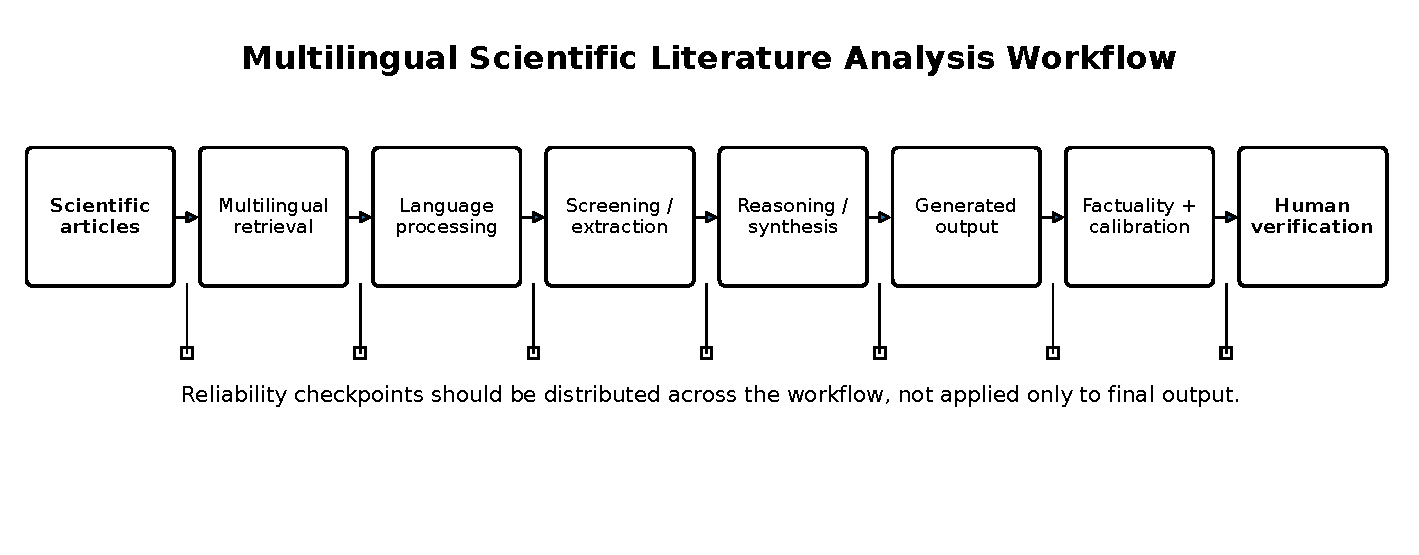
\includegraphics[width=0.98\textwidth]{figures/fig2_workflow.pdf}
\Description{A left-to-right scientific literature workflow from articles through multilingual retrieval, language processing, screening and extraction, reasoning and synthesis, generated output, factuality and calibration checking, and human verification.}
\caption{Multilingual scientific literature analysis workflow. Reliability checks should be distributed across retrieval, language processing, screening/extraction, reasoning, generation, and final verification.}
\label{fig:workflow}
\end{figure*}

\section{Research Challenges and Limitations}\label{sec:challenges}
Several methodological and practical limitations constrain what the current evidence base can support. First, multilingual benchmark construction introduces confounds because many benchmarks are created by translating English-language items. Differences in translation quality or construct equivalence can therefore contribute to an observed performance gap, and LLM-assisted benchmark construction can introduce circularity when similar systems are later evaluated on those items \cite{Xuan2025}.

Second, language coverage remains skewed toward languages with substantial digital resources. Benchmarks with dozens of languages still cover only a fraction of global linguistic diversity, while genuinely low-resource languages remain comparatively sparse in scientific evaluation \cite{Xuan2025,Qin2025}.

Third, most reliability research evaluates isolated tasks such as question answering, classification, or summarization rather than the full multi-step literature-analysis pipelines used in practice. A real workflow can retrieve candidate articles, screen them, extract evidence, synthesize findings, and generate a report. Errors can compound across these stages, while English-centric evidence-synthesis evaluations show that screening behavior is sensitive to the formulation of inclusion and exclusion criteria \cite{Scherbakov2025,DelgadoChaves2025}.

Fourth, the mitigation strategies in Section~\ref{sec:approaches} have their own dependencies. RAG depends on the availability of retrievable multilingual evidence; cross-lingual reasoning can transfer English-centric assumptions; and multilingual factuality metrics can inherit limitations from their supervision signals \cite{Qin2025,Huang2025,Lewis2020}.

Fifth, human evaluation remains difficult to scale across languages and specialized scientific domains. Bilingual domain experts are scarce, and automated evaluation can reproduce some of the same resource asymmetries that multilingual evaluation is intended to measure. These limitations motivate the research directions in Section~\ref{sec:gaps}.

\begin{figure*}[t]
\centering
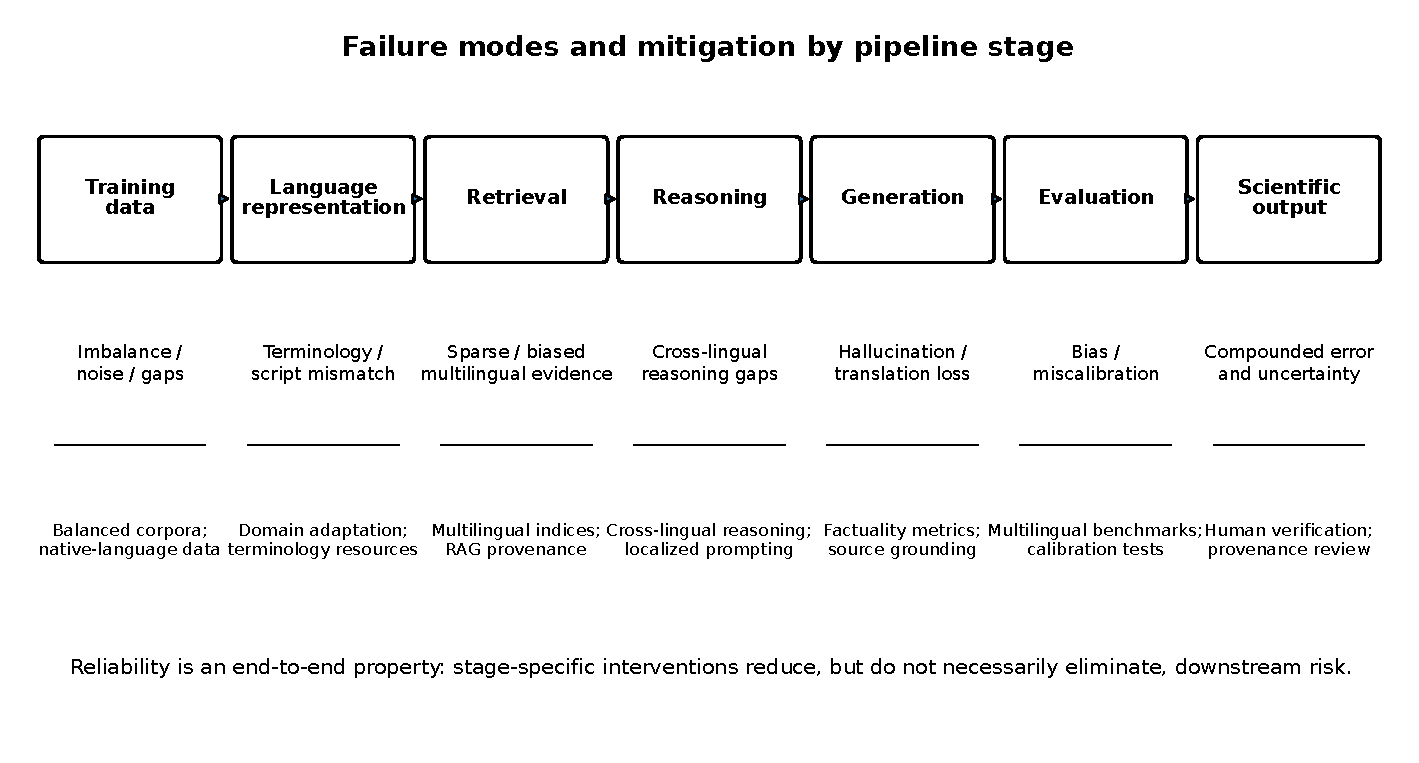
\includegraphics[width=0.98\textwidth]{figures/fig3_pipeline.pdf}
\Description{A pipeline showing training data, language representation, retrieval, reasoning, generation, evaluation, and scientific output, with reliability problems and mitigation strategies at each stage.}
\caption{Reliability degradation and mitigation across the scientific literature analysis pipeline. Each stage can introduce a distinct failure mode and requires a corresponding intervention; downstream human verification provides an additional safeguard.}
\label{fig:pipeline}
\end{figure*}

\section{Research Gaps and Future Directions}\label{sec:gaps}
Figure~\ref{fig:pipeline} frames the research gaps as an end-to-end pipeline problem. Table~\ref{tab:gaps} summarizes the major gaps and connects each to a concrete research direction.

\subsection{Standardized Evaluation and Low-Resource Coverage}
The field lacks a widely adopted protocol for evaluating multilingual reliability specifically within scientific-literature workflows. Future benchmark development should prioritize end-to-end pipeline evaluation, natively authored items where feasible, and error taxonomies that distinguish translation-induced errors from reasoning or factuality failures \cite{Huang2025,Xuan2025}.

Existing benchmarks concentrate on languages with larger digital text resources. Progress requires native-language scientific corpora, community-engaged terminology development, and evaluation designs that test locally relevant scientific knowledge rather than relying exclusively on translated English-source items \cite{Qin2025,Xuan2025}.

\subsection{Multilingual Retrieval, Calibration, and Uncertainty}
Because RAG depends on a retrievable knowledge base, multilingual scientific retrieval infrastructure is a direct reliability bottleneck. Research directions include multilingual embeddings, cross-lingual indices connecting non-English text with authoritative sources, and open multilingual scientific corpora \cite{Lewis2020}.

Given documented multilingual confidence differences, scientific systems should communicate uncertainty rather than present equally confident output regardless of language. Language-aware thresholds and interfaces that expose retrieval provenance and confidence estimates are potential directions grounded in the observed calibration problem \cite{Xue2024}.

\subsection{Structural Bias and Human-in-the-Loop Verification}
Language bias in scientific publishing predates LLMs and can interact with technical model limitations \cite{Amano2023}. Future work should therefore connect model evaluation with editorial and institutional interventions that reduce language-based barriers, rather than assuming that model improvements alone will resolve structural disparities.

No reviewed mitigation strategy eliminates multilingual reliability differences across all tasks and languages. Evidence-synthesis research already supports workflows in which LLM output augments rather than replaces expert screening \cite{Scherbakov2025}. Extending this principle to multilingual literature analysis suggests human verification should be explicitly integrated for claims or outputs whose provenance, calibration, or language-specific reliability is uncertain.

\begin{table*}[t]
\caption{Research gaps and future directions.}
\label{tab:gaps}
\scriptsize
\renewcommand{\arraystretch}{0.92}
\begin{tabularx}{\textwidth}{p{1.8cm}Y Y Y}
\toprule
Research Gap & Evidence/Problem & Consequence & Proposed Research Direction \\
\midrule
Standardized multilingual scientific evaluation & Benchmarks are often task-specific and frequently translated from English. & Cross-study comparisons are difficult and translation artifacts can confound results. & Develop end-to-end, natively authored multilingual scientific-literature benchmarks with explicit error taxonomies. \\
Genuinely low-resource language coverage & Existing benchmarks favor languages with larger digital corpora. & Reliability claims may not generalize to underrepresented language communities. & Build native scientific corpora and community-engaged terminology and evaluation resources. \\
Multilingual-native retrieval infrastructure & Lower-resource languages often have sparse indexed scientific evidence. & RAG cannot fully compensate for missing or inaccessible source material. & Develop multilingual indices, embeddings, linked evidence graphs, and open scientific corpora. \\
Calibration and uncertainty & Confidence estimation varies by language and task. & Users may misinterpret equally confident outputs as equally reliable. & Develop language-aware calibration, uncertainty thresholds, and provenance-aware interfaces. \\
Structural/linguistic bias & Scientific publishing and evaluation remain language-imbalanced. & Technical improvements may leave institutional language barriers intact. & Combine model evaluation with editorial, reviewer, and publication-process interventions. \\
Human-in-the-loop verification & Automated evaluation and generation remain imperfect, especially across languages and domains. & Unsupported claims can propagate into scientific synthesis. & Design multilingual workflows with explicit expert review triggers and provenance checking. \\
\bottomrule
\end{tabularx}
\end{table*}

\section{Conclusion}\label{sec:conclusion}
Large language models offer documented potential to reduce language barriers in scientific literature analysis, from translating scientific articles to supporting domain-specific question answering and evidence-synthesis tasks \cite{Kleidermacher2025,GarcíaFerrero2024,Scherbakov2025}. At the same time, the reviewed evidence shows that multilingual reliability is uneven. Performance differences appear in general multilingual benchmarks, biomedical question answering, confidence estimation, translation, and hallucination research, and these differences can affect multiple stages of a scientific workflow \cite{Hu2020,Xuan2025,GarcíaFerrero2024,Xue2024,Huang2025}.

The collective evidence supports an end-to-end view of reliability. Uneven training resources can affect representation; terminology and translation can alter evidence; retrieval can fail when multilingual corpora are sparse; reasoning and generation can introduce language-specific errors; and evaluation can conceal uncertainty if confidence is not calibrated across languages. Mitigation strategies such as RAG, multilingual factuality evaluation, cross-lingual reasoning, and domain adaptation can improve particular components, but their benefits remain conditional on data, retrieval, evaluation design, and language coverage \cite{Lewis2020,Qin2025,Qiu2024}.

For scientific literature-analysis workflows, the unresolved priorities are therefore clear: standardized task-realistic multilingual evaluation, stronger coverage of genuinely low-resource languages, multilingual-native retrieval infrastructure, calibration and uncertainty communication, attention to structural language bias, and explicit human verification. The central practical implication is not that multilingual LLMs should be excluded from scientific work, but that their outputs should be evaluated and verified in ways that reflect the language, domain, and workflow stage in which they are used.

\bibliographystyle{ACM-Reference-Format}
\bibliography{references}
\end{document}
